	Once selected the datasets, an exploratory data analysis has been carried out to understand the hidden properties between bands from the images and the images themselves to gather enough information and make the dataset comprehensible so that the design and evaluation of deep learning models can be more straight-forward. Moreover, the \gls{eda} was aimed to provide insights into potential challenges that might be encountered during the development of the model. This stage of the thesis proposed four main challenges:
\begin{itemize}
	\item Aggregating these datasets into a unified and standardized format is essential to ensure consistency and compatibility during the subsequent stages of the deep learning model development. Although both datasets are meant to be aggregated at some point, a solution to fit the dataset schema into the actual challenge was needed.
	\item Extracting the properties using various techniques, including image processing algorithms and statistical analysis, without getting away from the main topic and, then, attempting not to create biases while extracting the model metrics.
	\item Visualizing the data can provide valuable insights but a huge amount of data extracted can be messy and create a high computational demand. Research about high order libraries to visualize the data.
	\item Understanding the limitations of the datasets, such as noise, class imbalance, or variations in image quality, allowing for the identification of potential biases and the formulation of suitable mitigation strategies.
\end{itemize}
During the \gls{eda} phase, various techniques were employed to extract meaningful information from the dataset. Descriptive statistics were computed to gain a preliminary understanding of the distribution, central tendency, and spread of the data across different bands. This provided an overview of the range and variability of values within each band, allowing for an initial assessment of their significance.
By visually inspecting the images, patterns and trends specific to cloud formations must be discerned, aiding in the development of strategies to tackle cloud removal effectively. Furthermore, feature engineering techniques were explored to derive additional meaningful features from the dataset. This involved transforming, aggregating, or combining existing features to capture important characteristics of the data. After each information was discovered, this steps were not considered to be sequential but concurrent phases to incrementally learn and study the data. Therefore, the following subsections must be interpreted as chapters of a story of the analysis rather than separated and independent subsections.
\subsection{Properties extraction and visualization of the first dataset}
At first, creating a data exploration of \texttt{SEN12MS-CR} \cite{sen12mscr} was perfect as a first stemp since it is the most aligned dataset. Once extracted and analyzed the data, merging it to the other data was thought to be more straight-forward to understand. The feature extraction of the dataset last $38 h$ of computation.
\\
\\
As a general overview of the dataset, as mentioned before, the data is already split into training, validation and testing sets to compare between third-party models, as it can be seen in \ref{fig:eda-training-split}. For that reason, any new data can only be added to the training or validation sets. 
\begin{figure}[H]
	\centering
	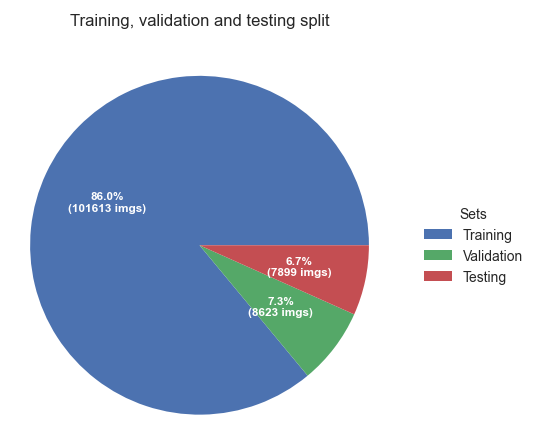
\includegraphics[width=9cm]{imgs/eda/split}
	\caption{Training-validation-testing split sets in SEN12MS-CR.}
	\label{fig:eda-training-split}
\end{figure}
An important step to take at this stage before processing, extracting features and visualize them was to take care of the pixel intensities in order to visualize and extract the information properly. The imagery values of each band were ranged from $0$ to $10000$. Therefore, the pixels need to be normalized and scaled for a proper processing and visualization of the data. This led to a challenge since the comparison or visualization of the properties extracted would be affected. Three normalization methods were thought:
\begin{itemize}
	\item MinMax Scaling, also known as feature scaling, is a method that linearly transforms the pixel values of an image to a specific range, typically between 0 and 1. 
	\[\text{Normalized value} = \frac{\text{Pixel value} - \text{Min Value}}{\text{Max value} - \text{Min Value}}\]
	Although this preserves the distribution of the pixel intensities of images for processing, this method is not proper for visualization since outliers can affect the visualization of the data, as it can be seen in \ref{fig:scaling-methods}. The max value must be the same for all the images ($1000$).
	\item Linear Stretch method. The linear stretch method is used to enhance the contrast of an image by stretching the pixel values across the a given available range.  If the pixel surpasses the 98\supindex{th} percentile, it will be 1 (or the maximum of the scaled vector). If the pixel value is under the 2\supindex{nd}, it will be 0 (or the minimum of the scaled vector). For the other pixel values, it performs the scaling operation by using interpolation, being the maximum value the 98\supindex{th} percentile and the 2\supindex{nd} the minimum.
	\[\text{Normalized value} = \frac{\text{Ranged pixel value} - \text{2\supindex{nd} percentile}}{\text{98\supindex{nd} percentile} - \text{2\supindex{nd} percentile}}\]
	\item Sigmoid after linear stretch method. The sigmoid after linear stretch method applies a sigmoid function to the linearly stretched pixel values to further enhance the contrast. In this formula, the slope $k$ is a parameter that controls the shape and position of the sigmoid function. The sigmoid function maps the stretched pixel values to a range between 0 and 1, enhancing the contrast in the process. By increasing the slope, the range of values can be compressed, so they get more blurred and with less contrast. This can be detected by applying the laplacian variance in the image. The slower the value, the higher its blurriness, as it can be seen in  \ref{fig:eda-laplacian-vars-slope} and \ref{fig:eda-sigmoid-slope}.
	\[\text{Normalized value} = \frac{1}{1 + e^{-k \cdot(\text{LinearStretch}(\text{Pixel value}))}}\]
	\begin{figure}[H]
		\centering
		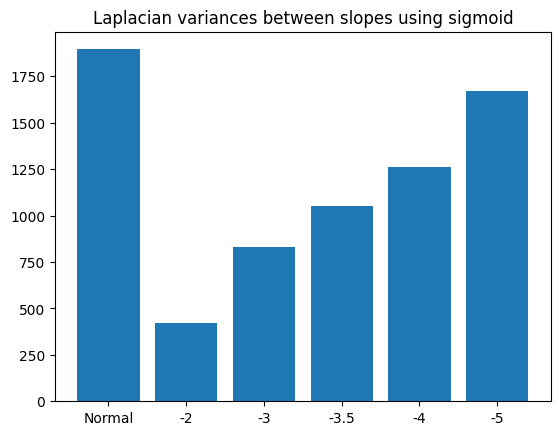
\includegraphics[width=9cm]{imgs/eda/sigmoid-slope-2}
		\caption{Laplacian variance depending on the slope used in sigmoid scaling method.}
		\label{fig:eda-laplacian-vars-slope}
	\end{figure}
\end{itemize}
The following pictures show how the images behave after treating each scaling method:
\begin{figure}[H]
	\centering
	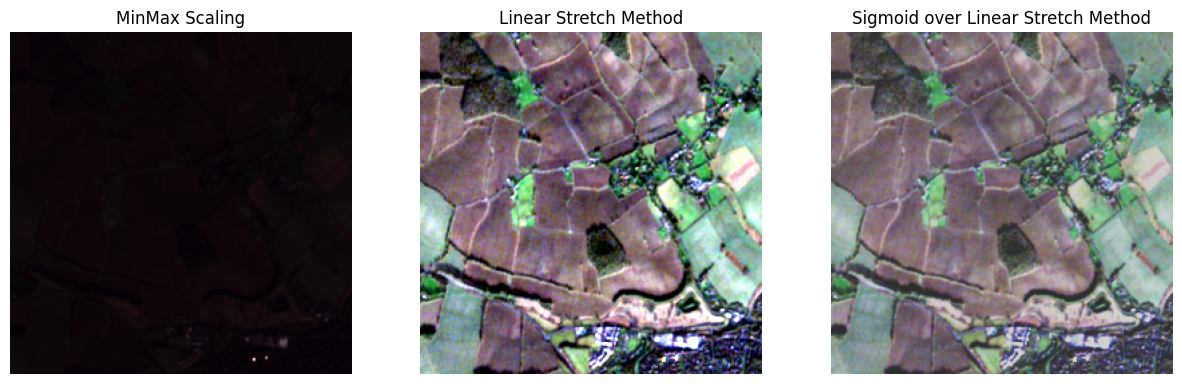
\includegraphics[width=15cm]{imgs/eda/scaled-methods-1}\\
	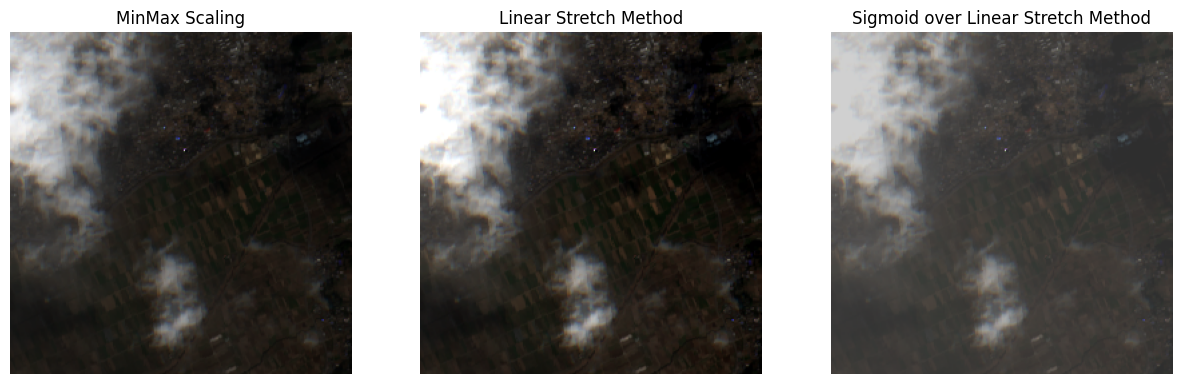
\includegraphics[width=15cm]{imgs/eda/scaled-methods-2}
	\caption{Scaling methods}
	\label{fig:scaling-methods}
\end{figure}
Regarding data processing for training, the best method to use is the MinMax feature scaling, since it preserves the intensity distribution and range of the values although its image visualization is poor.
\\
\\
Regarding data visualization and general data extraction, although it seems in \ref{fig:scaling-methods} that the best normalization to apply is sigmoid after the linear stretch method, we can see in \ref{fig:eda-sigmoid-slope} that this would affect the study of the properties since the data would be so compressed that the visual results could lead to confusion. Therefore, the best method to carry out while visualization is the linear stretch method, since there are some pixel intensities that are outliers due to the noise or other obstacles while capturing the images.
\begin{figure}[H]
	\centering
	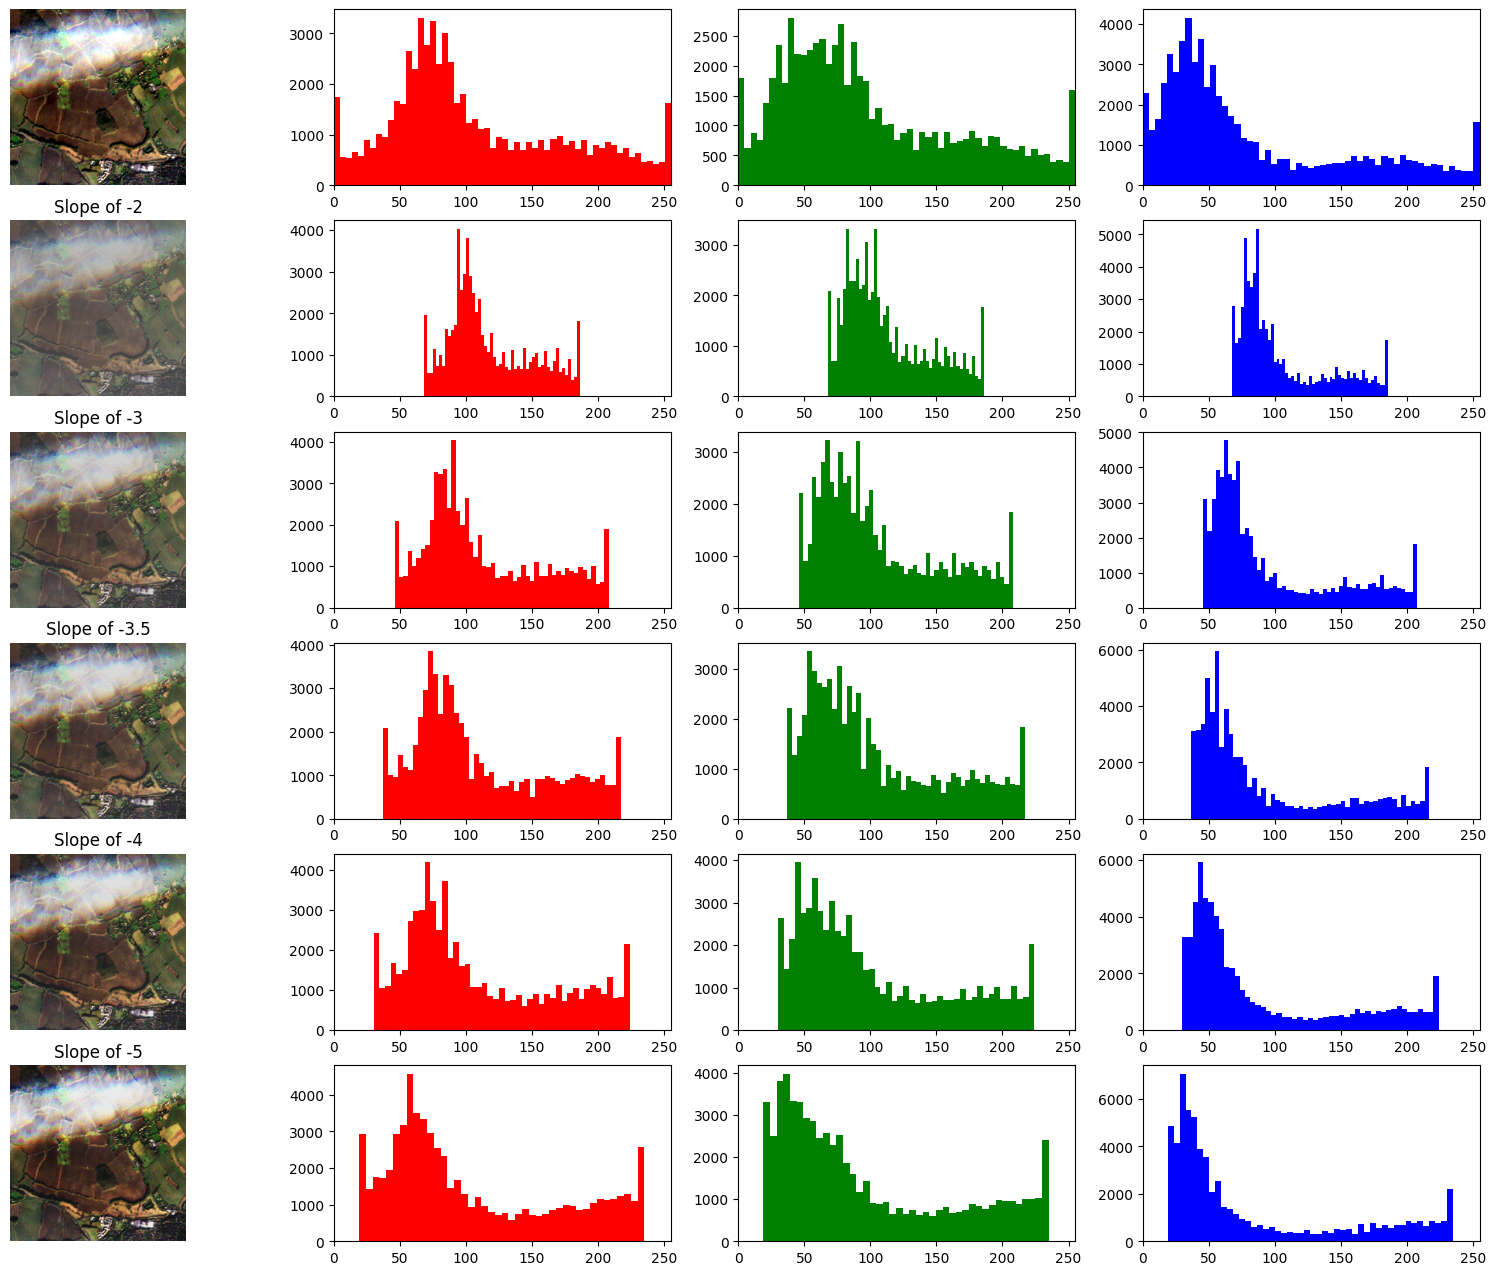
\includegraphics[width=16cm]{imgs/eda/sigmoid-slope}
	\caption{Sigmoid-scaled images with their RGB bands in different slopes.}
	\label{fig:eda-sigmoid-slope}
\end{figure}
The properties compared in the first dataset are classified depending on how they were extracted:
\begin{enumerate}
	\item Band properties of each image. Exploring properties related to individual bands helped to compare two bands given an image or different samples of images given these band properties. Since the data process changes the identification of the bands, in table \ref{tab:band-translation} is detailed the translation of the bandwidths.
	\begin{itemize}
		\item Descriptive statistics such as the mean, median, std and percentiles to compute  statistics for each band, providing insights into the distribution, central tendency, and spread of data values.
		\item Contrast. Analyzing the range and variation in pixel intensities within each band to understand the degree of contrast present. There are several ways to calculate contrast, the most popular ways are:
		\[\text{Traditional contrast} = \frac{\text{std}(\text{band})}{\text{mean}(\text{band})}\]
		\[\text{Michelson contrast} = \frac{\text{Maximum value} - \text{Minimum value}}{\text{Maximum value} + \text{Minimum value}}\]
		\item Blur. Assessing the level of blurriness in the images, indicating the sharpness of details captured. To extract the blurriness of the images, it has extracted the variance of the images after applying the laplacian filter.
		\item \gls{kde} helped to visualize the probability density function of each band, aiding in the identification of underlying patterns or modes.
	\end{itemize}
	\item True Color Image properties of each image. Although not all the bands captured from sentinel2 are visible in human spectra, comparing properties of the RGB bands could help us humans to understand the difference in the image captures.
	\begin{itemize}
		\item Saturation. Examining the saturation level of colors in the TCI, which indicates the vividness or intensity of hues. To get the saturation it has been changed from RGB to HSV color space.
		\item Temperature. Assessing the temperature or color balance of the TCI, providing information about the overall warmth or coolness of the image. To capture the temperature the images have been converted from RGB to CIE 1931 XYZ color space.
	\end{itemize}
	\item  The cloud coverage of each image was captured using the library  
	\begin{itemize}
		\item Percentage of each image. This quantifies the extent to which each image is covered by clouds, enabling the assessment of potential challenges posed by cloud interference.
		\item The MSE between cloud-free reference images and their corresponding cloudy versions was calculated allowing us for the evaluation of image quality degradation due to cloud cover.
	\end{itemize}
	\item An exploration of the indices showed in \ref{tab:sentinel2-bands} helped to reveal additional characteristics or features within the images and differences between the season and regions of interest.
\end{enumerate}
The analysis was ideal as a first step but hard to visualize due to the high amount of properties collected and its diversity of nature. Visualizations played a crucial role in revealing the inherent structure and characteristics of the dataset and for that reason, a first glance of the data should be done interactively. 
Since the variability of the cases where to compare the dataset and how extremely hard was to visualize correctly and effectively all the properties data extracted, the best decision to make was creating a web app to help the user experience of the \gls{eda}. To sum up, the goal of the app is to give a first glance of the dataset and find any imbalance. 
\\
\\
The app is powered by Streamlit. The library is a powerful and user-friendly python library that simplifies the process of building interactive web applications for data analysis and machine learning. It provides a straightforward way to create custom web interfaces directly from Python scripts, enabling users to easily visualize and explore data, create interactive dashboards, and share their work with others.
\\\\
Streamlit works by writing Python code that defines the various components of the web application, such as widgets, plots, and text. These components are then rendered in a web browser, creating an interactive user interface. The library takes care of handling the communication between the Python backend and the frontend, making it seamless for users to interact with the application. However, since the amount of data extracted from the images was huge, the efficiency of data processing while rendering the page decreases.
\\
\\
First of all, a sample of 100 images was extracted to visualize how is the variety of cloudy images. From \ref{fig:eda-first-exploration}, we can state that there are type of cloudy images:
\begin{itemize}
	\item Overcast images. These images show complete cloud cover, obscuring the land below.
	\item Mostly cloud, covering more than 75 \% of the land, allowing for some visibility but still showing significant cloud cover
	\item Partly cloud. A cloud that covers a big region of the image, between 25 \% and 75 \% of the land.
	\item Stratus clouds. Low, gray clouds covering the land like a blanket, often giving the image a dull appearance.
	\item Cumulus clouds. Puffy, small and white clouds dispersed over the image.
	\item Altostratus clouds. Clouds that there are in a high altitude and create a shadow in the land.
	\item Apparently clear. These are tricky cases where the cloud detection model might not be correct to identify as cloudless images. This could either mean a clear sky or a false negative from the model.
\end{itemize}
An ambiguity found in the dataset is that some data is not in any of the three set partitions, this could be due to the quality of them or the land cover changes in the region of interest, as it can be seen in \textit{Figure \ref{fig:eda-unclassified}}.  Therefore, they were not included in the training set.
\begin{figure}[H]
	\centering
	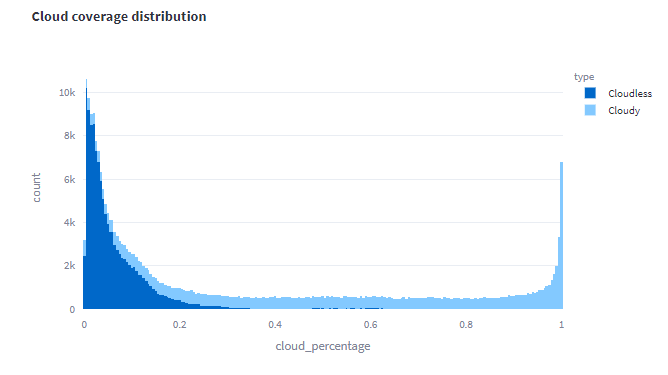
\includegraphics[width=16cm]{imgs/eda/cloud-coverage-distribution}
	\caption{Distribution of the dataset regarding the cloud cover percentage area}
	\label{fig:eda-cloud-percentage-area}
\end{figure} 
As figure \ref{fig:eda-cloud-percentage-area} shows, the dataset has a uniform constant distribution of cloudy images regarding its cloud covering area percentage without considering the peak of totally covered images. Therefore, the models trained would be less likely to remove clouds from a spcecific range or to be in a state of \textit{mode collapse}. It has been searched for those cloudy images with low cloud covering area. The problem is because of the blurriness of the images, as it can be seen in figures \ref{fig:eda-blurriness-images}, \ref{fig:eda-low-cloud-but-cloudy} and the scatter plot of cloudy images \ref{fig:eda-cloudy-images-blurred}. However, since there is only $1324$ blurred images\footnote{They represent less than a 1 \% of the total data.} and its \texttt{SAR} data is ok, it might be great to have them to allow the model also turn the noise into representative images but also to replicate former models mentioned in \textit{Section \ref{sec:soa}}.
\begin{figure}[H]
	\centering
	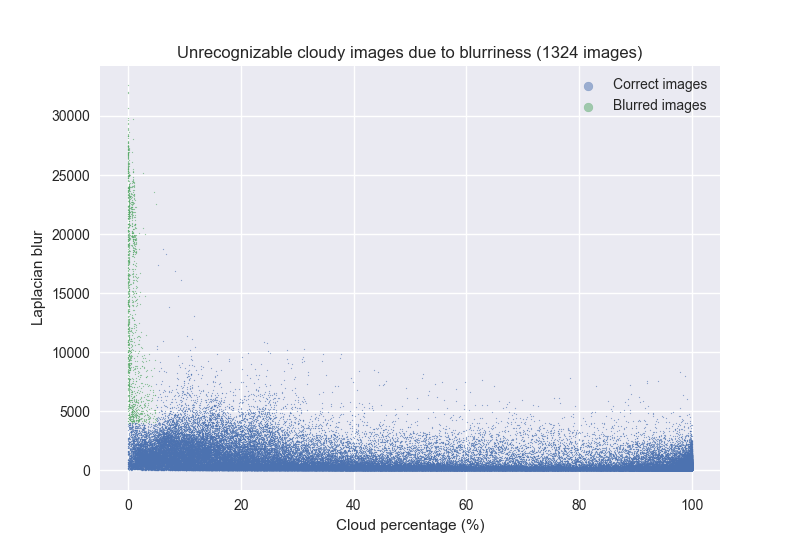
\includegraphics[width=16cm]{imgs/eda/cloudy-images-blurred}
	\caption{Sample of images labeled as cloudy but with low cloud cover percentage area.}
	\label{fig:eda-cloudy-images-blurred}
\end{figure} 
Regarding cloudless images, it can be seen in \textit{Figure \ref{fig:eda-cloud-percentage-area}} that they follow a heavy tail distribution, meaning that:
\begin{enumerate}
	\item[a)] our cloud detector model detects more false positives images
	\item[b)] there is a misleading tagging process in the dateset
\end{enumerate}
Moreover, some cloudless images have a high cloud area percentage. In this case, it is due to the haze, which our cloud detector identify these pixels as cloud but the acadamic dataset did not tag them as that, as it can be seen in \textit{Figure \ref{fig:eda-haze-cloudless}}.
\\
\\
That having been said, it is more than intuitive that blurriness affect the processing and evaluation of the dataset, although it is itself a characteristic of the dataset. In \ref{fig:eda-blurriness-images} it can be seen a sample of blurred images to demonstrate its gravity when it happens. A grosso modo, the blurriness in S2 can be caused \footnote{All these errors and more are listed in \cite{Sentinel2Anomalies}} by
\begin{itemize}
	\item atmospheric conditions, such as haze, aerosols, and clouds itself, since they absorb light reducing their clarity.
	\item satellite motion, if the satellite or the objects on the ground are moving rapidly during image capture, this can also be due to an atmospheric condition or mechanical vibrations.
	\item data processing. For example, some occurrences of yellow pixels over extra brights clouds have been identified when looking at the true color image visualization.
\end{itemize}
This effects do not only cause blurriness to the images but also particular changes in their saturation and temperature, as it can be seen in \textit{Figures \ref{fig:eda-scatter-blur-saturation} and \ref{fig:eda-scatter-temperature-saturation}}.
\begin{figure}[H]
	\centering
	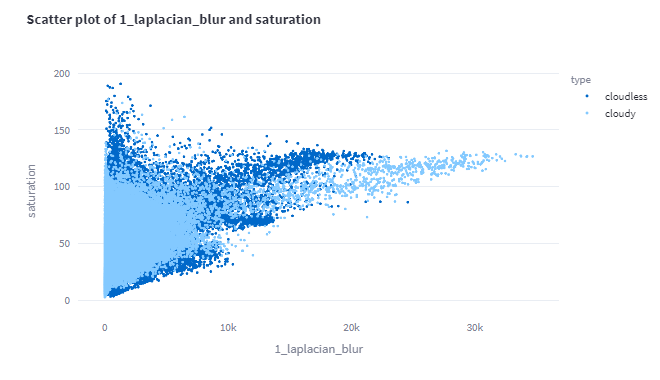
\includegraphics[width=13cm]{imgs/eda/blur-saturation}
	\caption{Scatter plot of the laplacian variance in B2 and the saturation of the true color image.}
	\label{fig:eda-scatter-blur-saturation}
\end{figure} 
\begin{figure}[H]
	\centering
	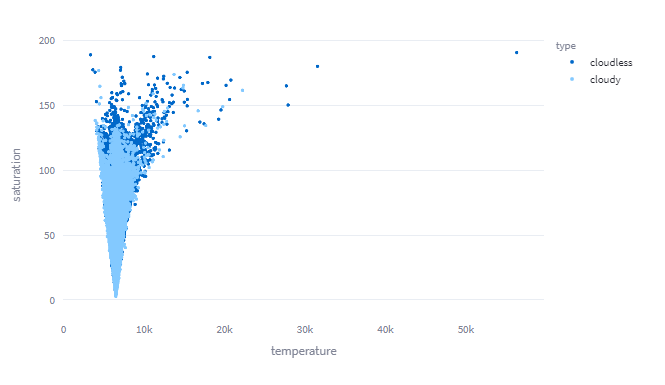
\includegraphics[width=13cm]{imgs/eda/saturation-temperature-outliers}
	\caption{Scatter plot of the temperature and the saturation of the true color image.}
	\label{fig:eda-scatter-temperature-saturation}
\end{figure} 
Moreover, Sentinel-2 includes a thermal infrared band (B10) that can be used to measure land surface temperature. High-temperature variations on the Earth's surface can lead to variations in thermal emissions, which may affect the quality of images in this band. We can see the difference of the bluriness in B1 and B10 regarding the saturation of the true color image checking \textit{Figures \ref{fig:eda-scatter-blur-saturation} and \ref{fig:eda-b10-blur-saturation}}.
\begin{figure}[H]
	\centering
	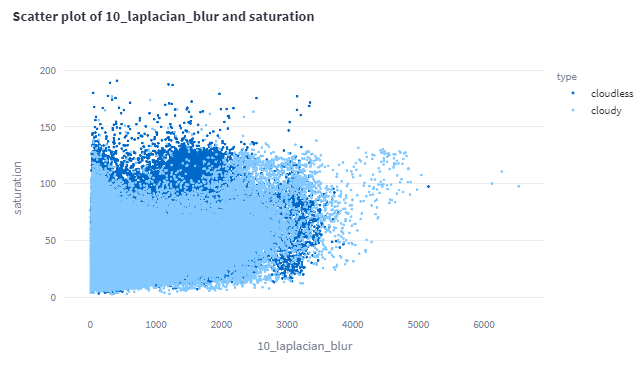
\includegraphics[width=13cm]{imgs/eda/b10-saturation-blurriness}
	\caption{Scatter plot of the laplacian variance in B10 and the saturation of the true color image.}
	\label{fig:eda-b10-blur-saturation}
\end{figure} 
Taking that into account, it has been decided how the B10 is affected by clouds comparing it with the other bands. First of all, it has been demonstrated that the bands are not affected equally to the clouds \ref{fig:eda-laplacian-blur}, being the true color images\footnote{B2, B2 and B3, showed as 1, 2 and 3 in \ref{fig:eda-laplacian-blur} respectively}, B8\footnote{Showed as 7 in \ref{fig:eda-laplacian-blur}.} and B10. Therefore, it has been decided not to employ perlin noise to create synthetic images with clouds, since this would lead to a bias in generating images.
\begin{figure}[H]
	\centering
	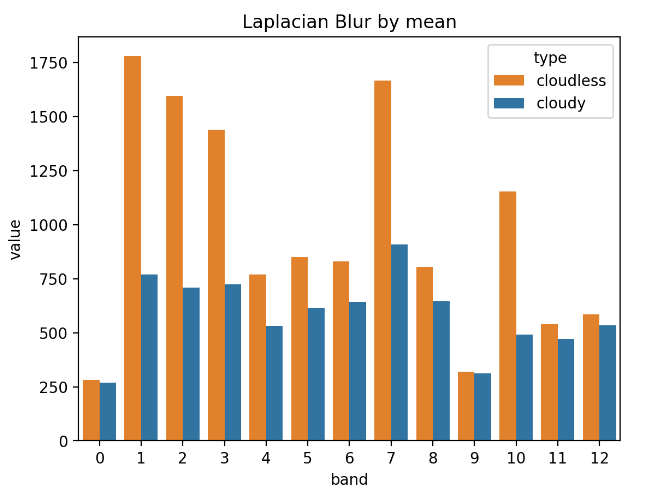
\includegraphics[width=9cm]{imgs/eda/laplacian-blur}
	\caption{Bar plot of the mean value in each band of the laplacian variance.}
	\label{fig:eda-laplacian-blur}
\end{figure}
Although this similarity in the TCI bands and B10, the blurriness does not behave equally regarding other properties from the image, e.g. the contrast, as it can be seen in the comparison of figure \ref{fig:eda-comparison-b1-b10}.
\\
\\
Moreover, in figure \ref{fig:eda-crop-correlation-b10} it is clear that there is a high correlation between the region affected by clouds and the values of B10, meaning that cloud regions cause high values of B10. However, not otherwise, as it shows \ref{fig:eda-mask-correlation-b10}.
\begin{figure}[H]
	\centering
	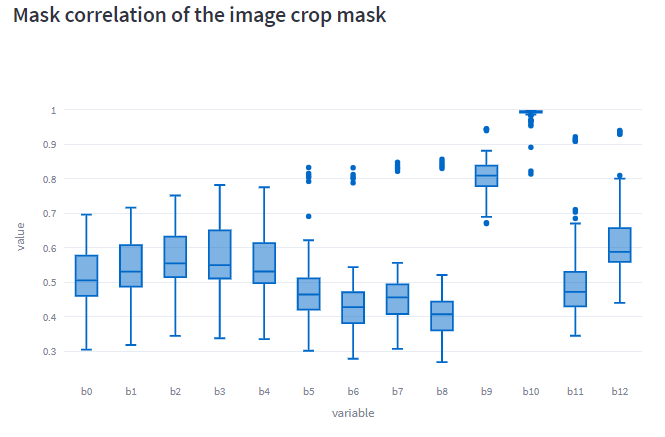
\includegraphics[width=11cm]{imgs/eda/crop-correlation}
	\caption{Correlation of the region with clouds and the values of the band, by mean from each image.}
	\label{fig:eda-crop-correlation-b10}
\end{figure}
The cloudy crop correlation did lead to ask how B10 behaves in cloudless and cloudy image respectively. By visualizing the kernel density estimation of B10 \ref{fig:eda-b10-kde} and the other ones\footnote{For instance, figure \ref{fig:eda-b3-kde}}, it is totally clear that B10 is the most corrupted and affected bandwidth by the presence of clouds. Therefore, a single metric to check the difference between the B10 of synthetic data and cloudless data could be helpful to discern the effectiveness of the models.
\begin{figure}[H]
	\centering
	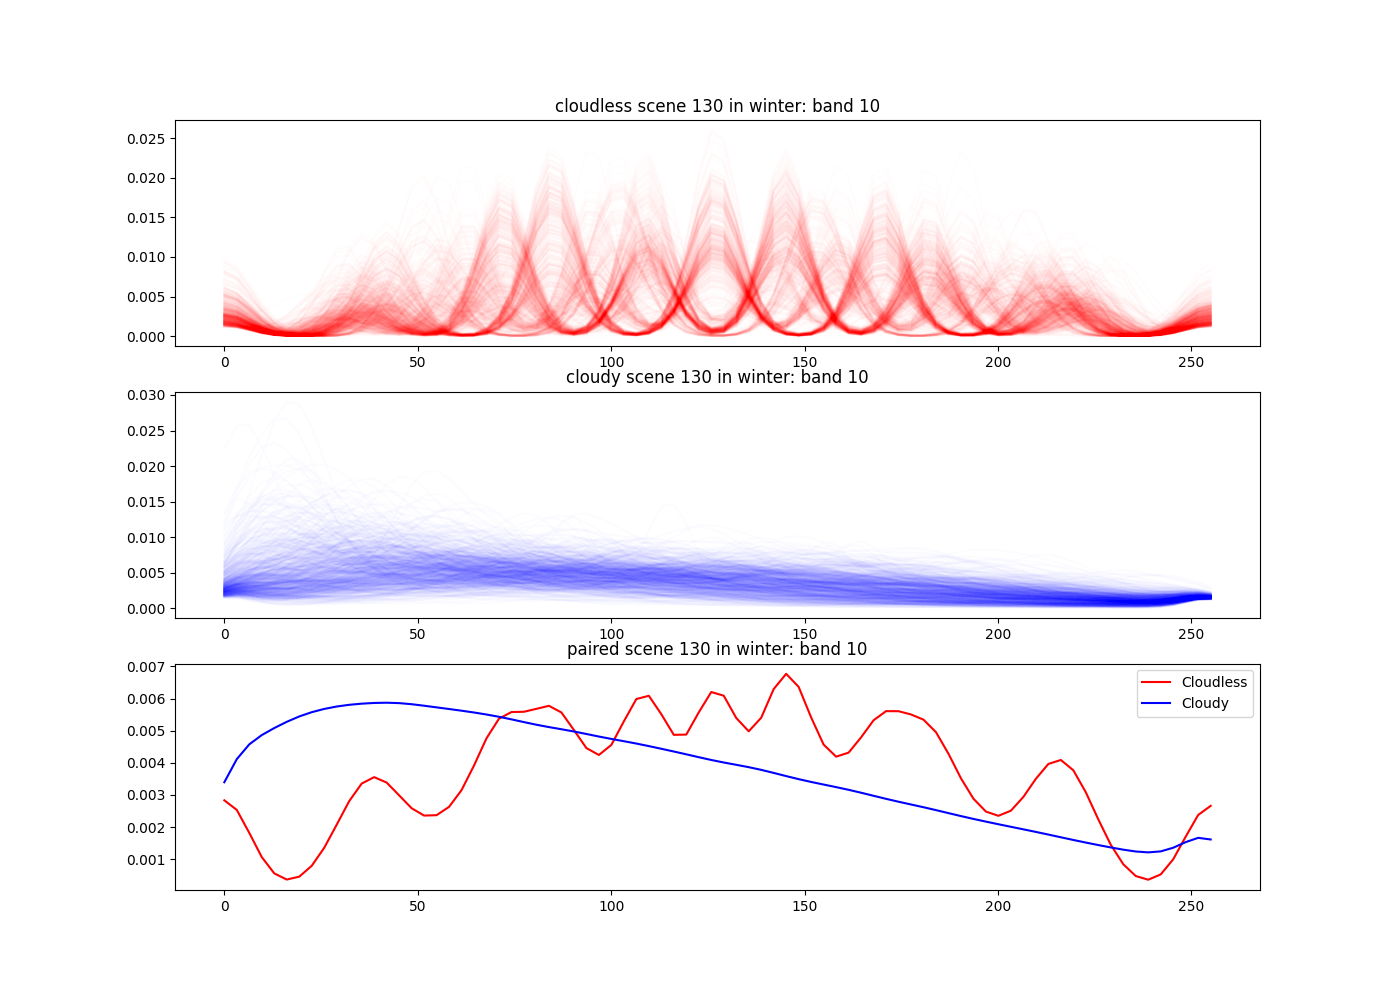
\includegraphics[width=16cm]{imgs/eda/b10-kde}
	\caption{Kernel density estimation of B10 in cloudy and cloudless the patches of a specific scene (130)}
	\label{fig:eda-b10-kde}
\end{figure}
Finally, it has been decided to include the blurry images in the training set to make the model robust against such real-world imperfections. Features to capture blurriness, saturation, and temperature could be engineered and fed into the model to improve its predictive power. For example, make the blurriness, the contrast and the temperature be in concordance from the target set.
Given the high sensitivity of B10 to cloud presence, incorporating a metric that compares the B10 values between synthetic and cloudless data, as suggested, should be useful to evaluate the model's performance specifically in terms of its handling of cloud-related features. Given that different bands react differently to clouds, a multi-modal neural network could be beneficial. Separate branches of the network could specialize in learning features from different bands and then combine them for final predictions.
